\section{Results}
\label{sec:results}

Here, we investigated fast adaptation in the mouse retina under natural
stimulus conditions. To this end, we trained a CNN model on RGC responses to a
movie of flashed images appearing naturally in the mouse environment,
% and then performed a model-guided
% search for stimuli that maximize the responses of RGCs.

\textbf{A method to estimate how selectivity to natural images changes over
    time.}
We recorded retinal ganglion cells (RGCs) in the mouse retina with
multi-electrode arrays (MEAs) while displaying sequences of natural images.
Each image was presented for 400 ms, preceded by one of three 400 ms adaptation
light patterns: grey, checkerboard, or inverted checkerboard (Figure
\ref{fig:CellExample}).
Each pair of adaptation patterns and natural images forms a stimulus clip
lasting 800 ms.
To measure the selectivity of RGC to different parts of the image, we added dim
checkerboard patterns (Figure \ref{fig:LSTA}).
The amplitude of the perturbation checkerboard was selected to introduce a
small yet visible change in the RGC response compared to the RGC response to
the unperturbed natural image.

For each cell and each stimulus clip, we computed an estimation of the local
spike-trigger average (LSTA) (Figure \ref{fig:CellExample}), as the average of
the
perturbation patterns weighted by the number of spikes they evoked. This
estimation is similar to a more classical Spike Trigger Average (STA) but due
to the small amplitude of the perturbation checkerboard, we explore here a
small, local region of the stimulus space centered on the reference natural
image. The LSTA is a visualization of the gradient of the RGC response at the
reference natural image point in stimulus space. From an experimental point of
view, instead of perturbating the biological system itself (e.g. shutting down
neuronal pathways), we perturbated the stimulus itself.
1000 repetitions with different perturbation patterns were necessary to
estimate the LSTA to one clip (see Methods).

We recorded RGC responses from four different eyes. The first experiment was
discarded since 750 repetitions were not sufficient to estimate the LSTA. The
second experiment was also discarded since the retina was very unhealthy during
the recordings. The third experiment was a great success with over 100 cells
showing relevant LSTA for many different clips. Finally, we used a fourth
experiment to both train and test a convolutional neural network and measure
LSTA, once again with
great success with about 100 cells with LSTAs despite the longer experimental
time.

\par~\textbf{Ganglion cells can change their selectivity depending on previous
    light patterns.}
We looked at the firing rate and the LSTA of more than 200 cells changed
depending on the adaptation light pattern. Some clear hypotheses can be made as
described in Figure \ref{fig:CellExample}. Adaptation effects can already be
seen in the temporal profiles of the responses.

As for the spatial effect on the LSTA, a first hypothesis would be that for On
cells, an area that stays white provokes less response than an area that goes
from black in the
adaptation pattern to white in the natural image (Figure \ref{fig:CellExample},
On cell, column 1) - respectively black for
Off cells (Off Cell, column 2,3). However, this hypothesis does not hold true
in all cases (On
cell, column 3). For OnOff cells, this adaptation can happen in both pathways
simultaneously
(Cell OnOff, column 1,2). We observed that a high spiking rate was not
necessarily linked with
a clearly defined LSTA and vice-versa.

It seems that in most cases, this observed displacement of the LSTA could be
explained by
the biphasic temporal dynamic of units of the LNLN model (Figure
\ref{fig:retina_structure}). For instance, if ON
bipolar cells are probed with white, they could be in the negative phase of
their
biphasic responses when the natural image appears which would reduce their
response. As a chained consequence, the associated RGC will receive less
excitation from that part of the image, which would cause the displacement of
the LSTA. Still, a single RGC can behave differently depending on the content
of the natural image, which would not be captured by an LNLN model with fixed
parameters.

We also noticed that the past natural image shown 800 ms before the current
natural image influenced
the response of the RGC to the current natural image. After looking at all the
PSTH of all the cells, we judged that it was minor enough to not impact the
behavior of the RGC that we wanted to visualize. Longer time windows would
reduce the number of repetitions that can be shown in a set amount of time and
reduce the quality of the estimation of the LSTA.
We have yet to do a statistical analysis of the number of occurrences of those
different behavior.

\begin{figure}
    \centering
    \vspace*{-3cm}
    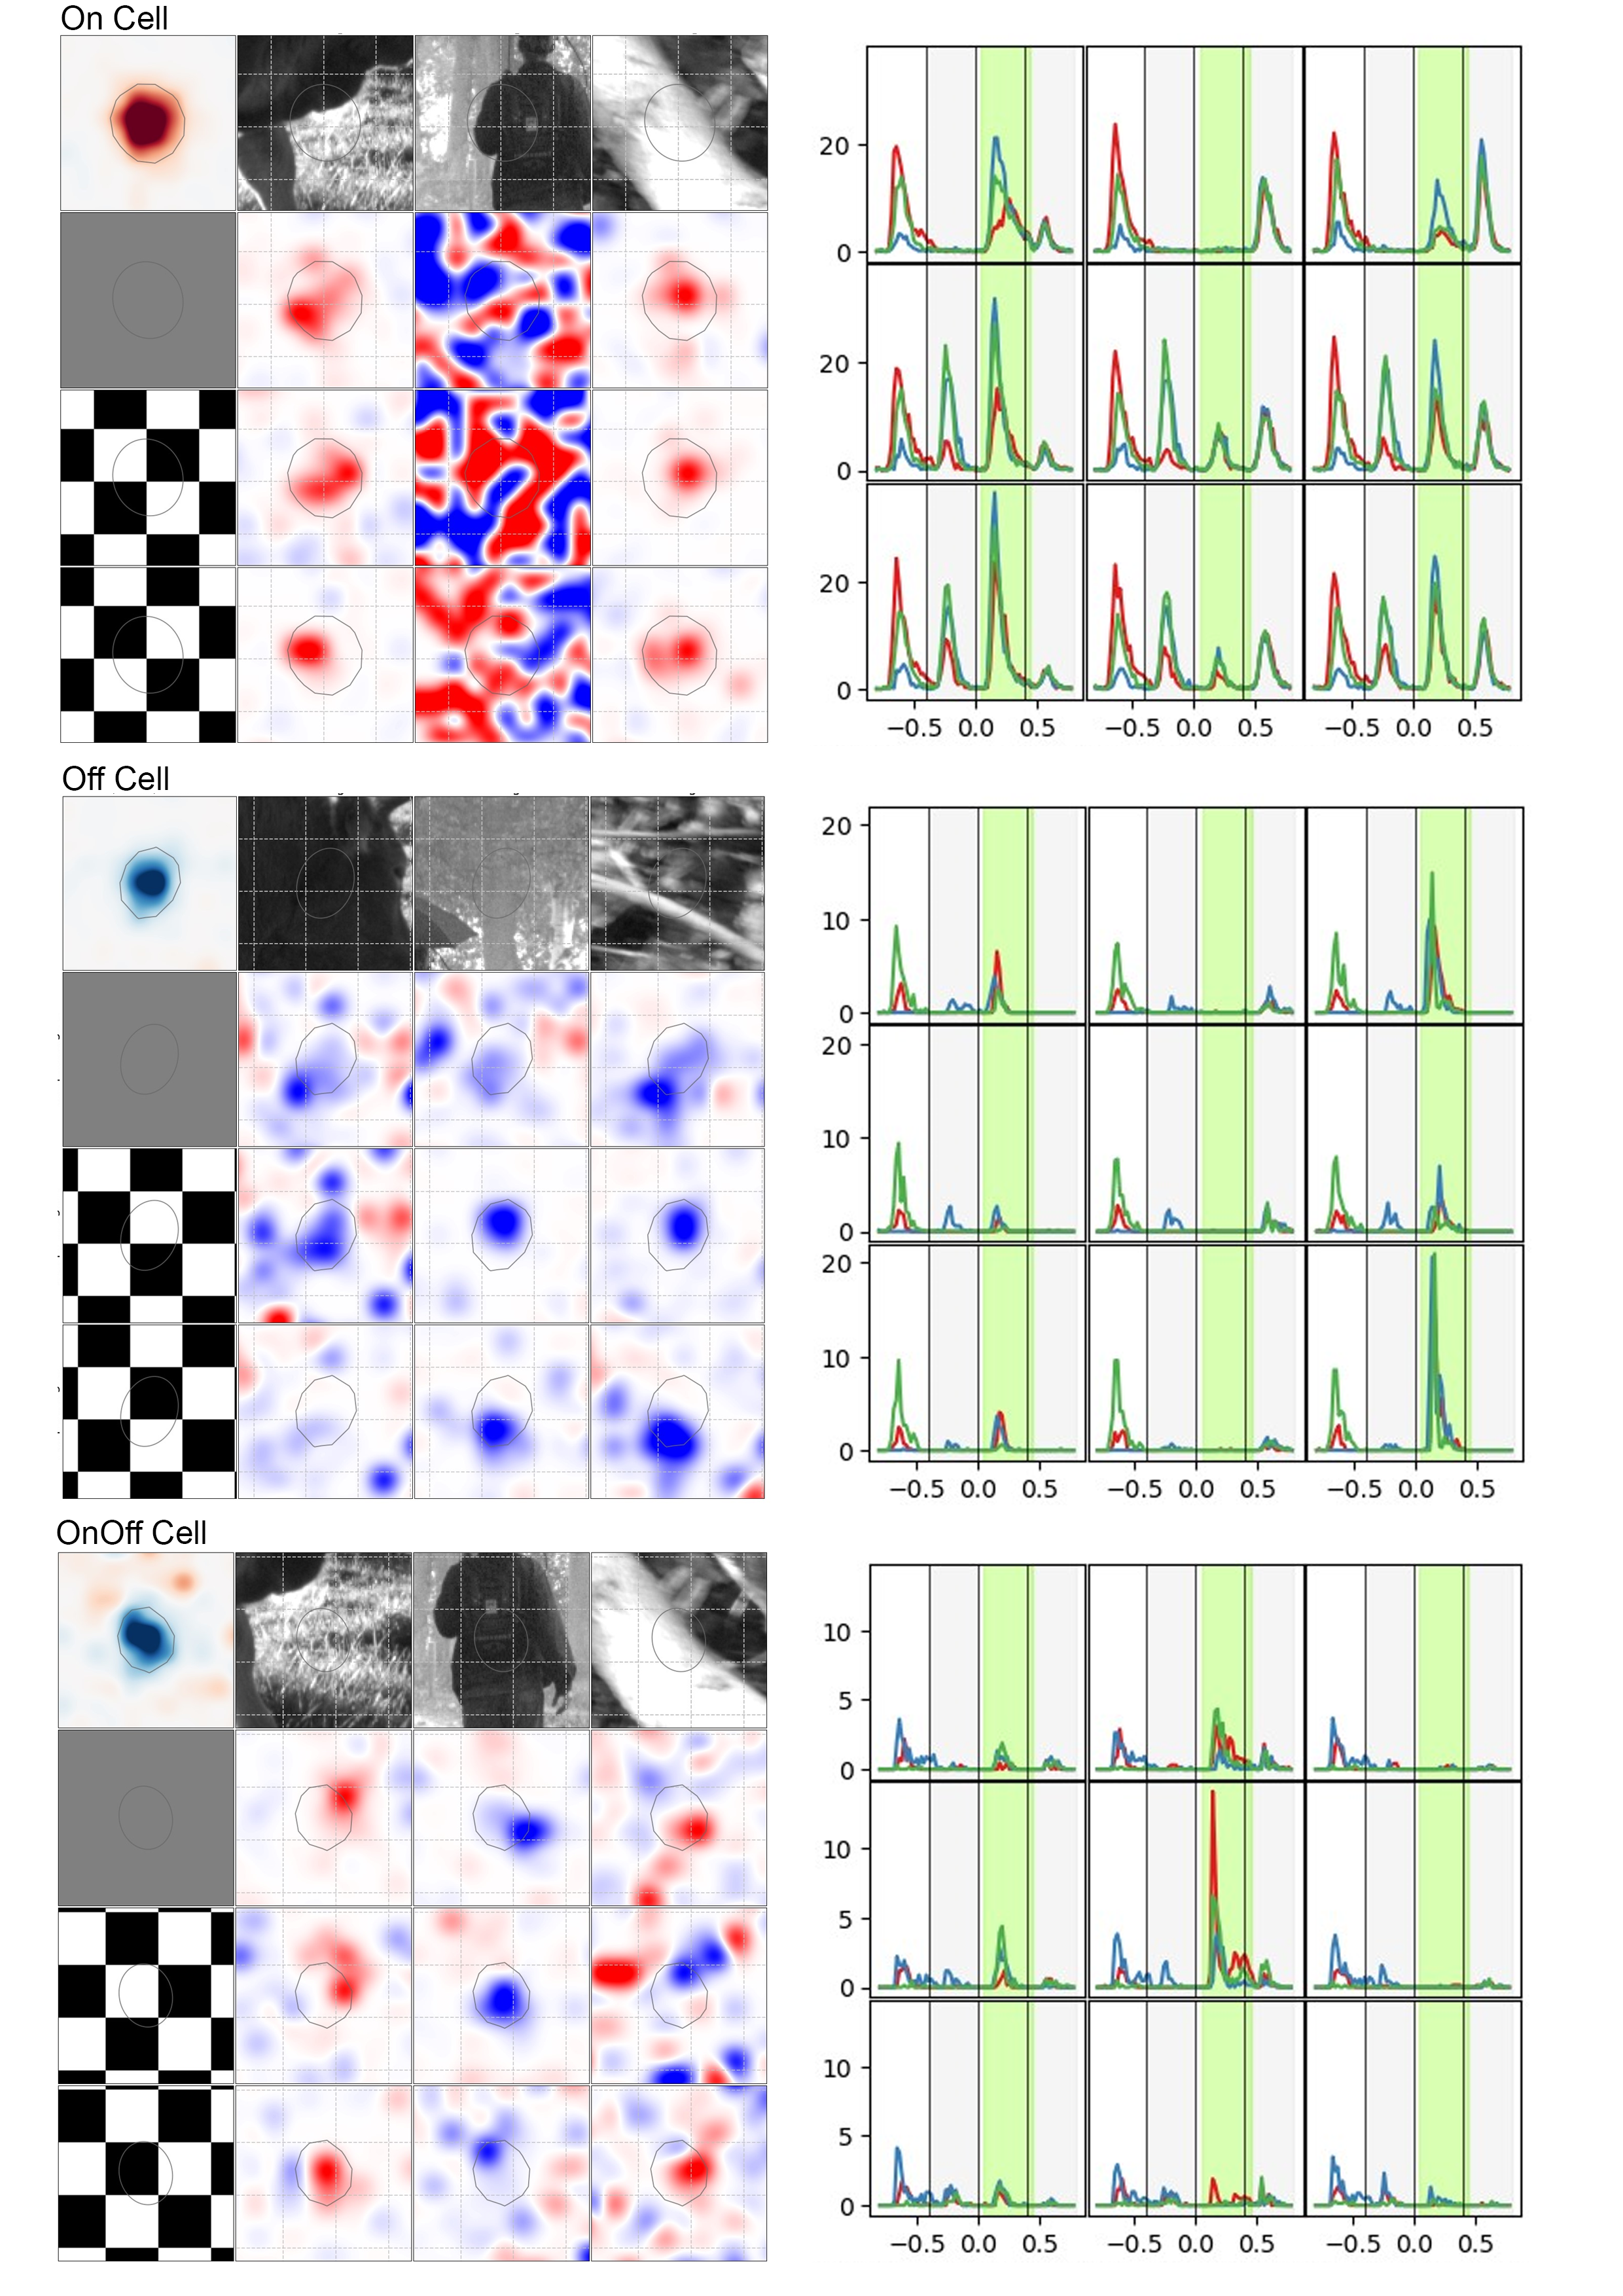
\includegraphics[width=0.8\textwidth]{pics/ExamplePSTHLSTA.png}
    \caption{\textbf{Temporal and spatial aspects of the response depend on
            previous light patterns: some
            exemplary RGCs.} \small	   \textbf{Left} Local Spike Triggered
        Average (LSTA), the average of the
        perturbation checkerboard patterns weighted by the number of spikes
        they
        evoked. Here we centered the view on the RGC receptive field and
        smoothed the
        LSTA using exponential tuning and spatial interpolation. We also
        display the STA in the top-left corner.
        \textbf{Right} Poststimulus time histograms
        (PSTH) are
        histograms of the times at which neurons fire.
        The disposition of the graph follows the same pattern as on the left.
        In each plot, the time
        bins in
        grey corresponds to the display of an adaptation pattern while time
        bins
        in
        white natural images.
        The time axis is centered on the moment when the current natural image
        is displayed. So in order the four rectangles are the previous natural
        image,
        current adaptation pattern, current natural image, and next adaptation
        pattern.
        The area highlighted in yellow corresponds to the 400 ms windows over
        which
        spikes are integrated to compute the LSTA.
        Each color corresponds to a different 'previous natural image'
        displayed 800ms before the current natural image.}
    \label{fig:CellExample}
\end{figure}

\textbf{Can a convolutional neural network model account for this dependence?}
We trained a convolutional neural network (CNN) model to predict the RGC
response to natural images. We hope to infer some of the governing
non-linearities in the recorded RGC. We expect the CNN model to have
good test performance on clips using the gray adaptation since it is trained on
such data However it's unclear how it will generalize to the other two
adaptation patterns. Additional divisive dynamics such as gain control would
have to be added to the model. More on model design can be found in Methods and
Appendix.

Here, we will show the results obtained from one of our models on one single
cell.
First, as we expected, the model predicted the clip using the gray adaptation
better and mostly failed in the other two cases (Figure
\ref{fig:CNNResults}.a). Notice that in most cases it
did predict a response but did not account for the new delay.
This hints at temporal dynamics being not well encoded in the CNN model.

However, test performances are not enough to validate a model that can be used
to build a hypothesis on the retinal code. We also have to make sure that the
model learns its filters to look like those of retinal cells. In the subunit,
we expect a center/surround spatial filter with a biphasic temporal filter. In
the RGC, we expect a localized receptive field, preferentially with a
center/surround spatial filter with a biphasic temporal filter. As shown in
Figure \ref{fig:CNNResults}.b, while the chosen model has a localized RGC
receptive field
with a slightly biphasic temporal filter, it lacks a clear surround in the
filter
of its subunits. As a consequence of the filters being too small, there are
large discontinuities on the border of the subunit filters that are not
desirable.
The structure of the filters is influenced by the L1 and L2 regularization that
are difficult to find tuned.

Finally, we would like to know if the CNN model can predict the displacement of
the LSTA observed before. We computed the LSTA as the average gradient of the
model over the frame of the stimulus that contained the natural image. This computation method is still in development. It seems
that the current model is not able to predict this displacement (Figure
\ref{fig:CNNResults}.c). This could
indicate that it structurally can't learn them, which would go in favor of
extending the model with more complex temporal dynamics such as gain control.
But it could also mean that the model was not properly trained.

\begin{figure}
    \centering
    \vspace*{-3cm}
    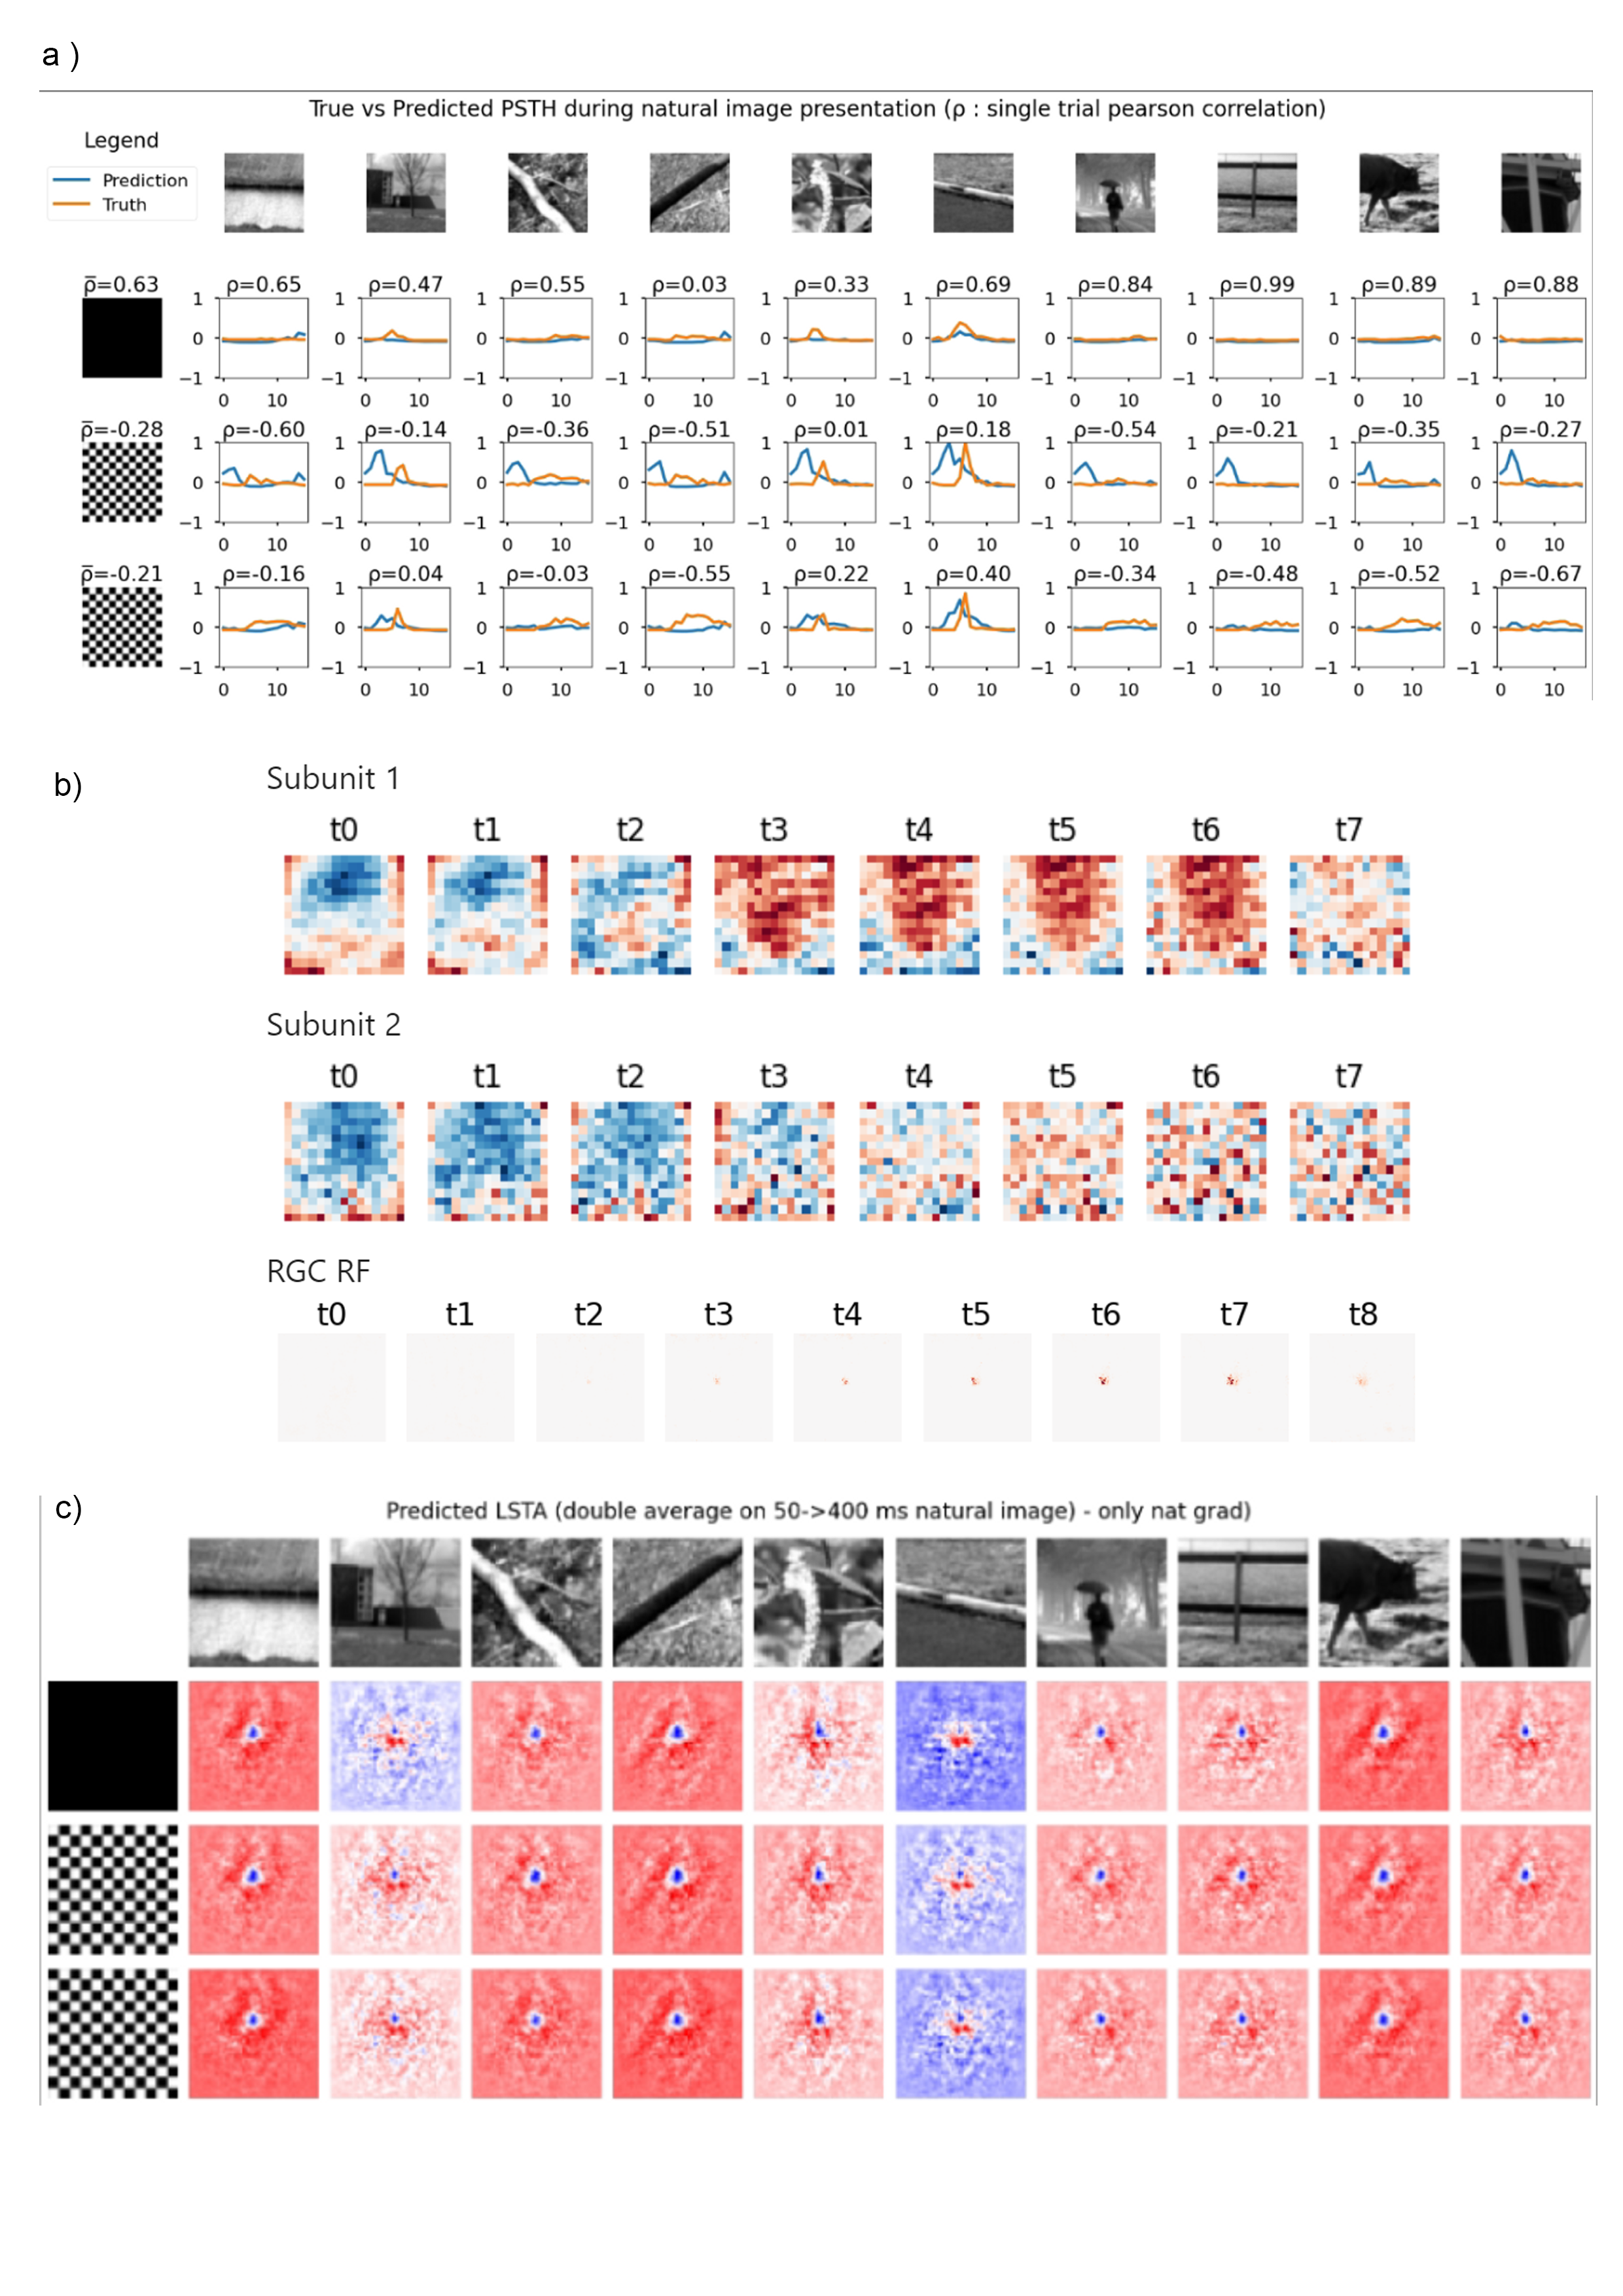
\includegraphics[width=\textwidth]{pics/CNNResults.png}
    \caption{\textbf{Resluts from the CNN model.} \textbf{a.} Single trial
        correlation $\rho$ performance
        of the CNN model on the three different adaptation patterns (see
        Methods). The model
        was
        trained on the gray adaptation pattern. \textbf{b.} Filters of the
        subunits and
        RGCs of the CNN model. \textbf{c.} LSTA computed from the CNN model.}
    \label{fig:CNNResults}
\end{figure}

\clearpage